\documentclass[11pt]{article}
\usepackage{setspace}
\setstretch{1}
\usepackage{amsmath,amssymb, amsthm}
\usepackage{graphicx}
\usepackage{bm}
\usepackage[hang, flushmargin]{footmisc}
\usepackage[colorlinks=true]{hyperref}
\usepackage[nameinlink]{cleveref}
\usepackage{footnotebackref}
\usepackage{url}
\usepackage{listings}
\usepackage[most]{tcolorbox}
\usepackage{inconsolata}
\usepackage[papersize={8.5in,11in}, margin=1in]{geometry}
\usepackage{float}
\usepackage{caption}
\usepackage{esint}
\usepackage{url}
\usepackage{enumitem}
\usepackage{subfig}
\usepackage{wasysym}
\newcommand{\ilc}{\texttt}
\usepackage{etoolbox}
\usepackage{algorithm}
\usepackage{changepage}
% \usepackage{algorithmic}
\usepackage[noend]{algpseudocode}
\usepackage{tikz}
\usetikzlibrary{matrix,positioning,arrows.meta,arrows}
\patchcmd{\thebibliography}{\section*{\refname}}{}{}{}
% \PassOptionsToPackage{hyphens}{url}\usepackage{hyperref}

\providecommand{\myceil}[1]{\left \lceil #1 \right \rceil }
\providecommand{\myfloor}[1]{\left \lfloor #1 \right \rfloor }
\providecommand{\qbm}[1]{\begin{bmatrix} #1 \end{bmatrix}}
\providecommand{\qpm}[1]{\begin{pmatrix} #1 \end{pmatrix}}
\providecommand{\norm}[1]{\left\lVert #1 \right\rVert}
\providecommand{\len}[1]{\left| #1 \right|}

\begin{document}



\title{\textbf{MATH 307: Individual Homework 9}}


\author{Shaochen (Henry) ZHONG, \ilc{sxz517@case.edu}}

\date{Due and submitted on 03/08/2021 \\ Spring 2021, Dr. Guo}
\maketitle



\subsection*{Problem 1}
\textit{See HW instruction.}\newline

Known that $<u, v> = \sum\limits_{i=1}^{3} u_i \overline{v_i}$ for $u, v \in \mathbb{C}^3$. We have the induced norm to be:

\begin{align*}
    \norm{u} &= \sqrt{\sum\limits_{i=1}^{3} u_i \overline{u_i}} \\
    &= \sqrt{\sum\limits_{i=1}^{3} \len{u_i}^2} = \norm{u}_2
\end{align*}

And we have the norm of $u = \qbm{1+i \\ 2i \\ 3+i}$ being:

\begin{align*}
    \norm{u}_2 &= (\sum\limits_{i=1}^{3} \len{u_i}^2)^{\frac{1}{2}} = \sqrt{\sum\limits_{i=1}^{3} \len{u_i}^2} \\
    &= \sqrt{(1^2 + 1^2) + (2^2) + (3^2 + 1^2)} = \sqrt{2 + 4 + 10} \\
    &= \sqrt{16} = 4
\end{align*}

For the distance between given $u, v$, we have:

\begin{align*}
    d(u, v) &= \norm{u - v} = \norm{\qbm{i \\ -3 + 3i \\ 3 + 2i}} \\
    &= \sqrt{1^2 + ((-3)^2 + 3^2) + (3^2 + 2^2)} \\
    &= \sqrt{1 + 18 + 13} = \sqrt{32} = 4\sqrt{2}
\end{align*}

\subsection*{Problem 2}
\textit{See HW instruction.}\newline

Since $x \in \mathbb{R}^2$ we have $x = [x_1, x_2]$ for $x_1, x_2 \in \mathbb{R}$.

\begin{figure}[H]
    \centering
    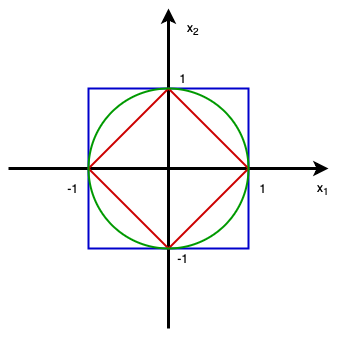
\includegraphics[width=0.5\linewidth]{{fig/fig_p2.png}}
    \caption*{Plots of \textcolor{red}{1-}, \textcolor{green}{2-}, and \textcolor{blue}{$
    \infty$-}norm unit balls in $\mathbb{R}^2$}
\end{figure}

\begin{itemize}
    \item \textbf{1-norm}: $\len{x_1} + \len{x_2} = 1$. Thus, we have all the points on the \textcolor{red}{red diamond} to be the unit ball of 1-norm.
    \item \textbf{2-norm}: $\sqrt{\len{x_1}^2 + \len{x_2}^2} = 1 = \len{x_1}^2 + \len{x_2}^2$. Thus, we have all the points on the \textcolor{green}{green circle} to be the unit ball of 2-norm.
    \item \textbf{$\infty$-norm}: $\max(x_1, x_2) = 1$. Thus, we have all the points on the \textcolor{blue}{blue square} to be the unit ball of $\infty$-norm.
\end{itemize}

For $x \in \mathbb{R}^2$ where $\norm{x}_1 = \norm{x}_2 = \norm{x}_{\infty} = 1$, we must look at the intersections of the \textcolor{red}{red}, \textcolor{green}{green}, and \textcolor{blue}{blue} plots -- which are $\{(1, 0), (0, -1), (-1, 0), (0, 1)\}$.


\end{document}

